% LaTeX Beamer From Scratch
%%
% Andre Pereira andrespp at gmail dot com
% 13/10/2009
%
% This document is based on the Beamer User Guide, available at:
% http://www.ctan.org/tex-archive/macros/latex/contrib/beamer/doc/beameruserguide.pdf

\documentclass{beamer}

%%%Style setup
%\usetheme{Madrid} 	% Very clean
%\usetheme{Antibes}	% 3 top bars: section, subsection, subsubsection
\usetheme{Frankfurt}	% 2 top bars: section, slide counter %%esse
%\usetheme{Ilmenau}
%\usetheme{Berlin}	% 2 top bars: section, slide counter
%\usetheme{Warsaw}	% large top bar
%\usetheme{Bergen} 	% left side bar (uhhg)
%\usetheme{Rochester} 	% clean with large top bar
%\usetheme{Darmstadt}
%\usetheme{Boadilla}	% super clean
%\usetheme{Copenhagen}
%\usetheme{Dresden}	% 2 top bars
%\usetheme{Malmoe}
%\usetheme{Goettingen}	% clear right bar
%\usetheme{Hannover}	% clear left bar
%\usetheme{Ilmenau}
%\usetheme{JuanLesPins}	% 3 top bars (slim)
%\usetheme{Luebeck}
%\usetheme{Marburg}	% bold right bar
%\usetheme{PaloAlto}	% left / top bar
%\usetheme{Singapore}	% clear top bar
%\usetheme{Szeged}
%\usetheme{default}	% totaly white background
%\usetheme{Montpellier}

%\usecolortheme{seahorse}	%diminui o contraste
%\usecolortheme{rose}			%diminui o contraste
%\usefonttheme[onlylarge]{structuresmallcapsserif}

% Hide slide bullets on header
\setbeamertemplate{headline}
 {%
  \begin{beamercolorbox}{section in head/foot}
  \insertsectionnavigationhorizontal{\textwidth}{}{}
  \end{beamercolorbox}%
}


%%%Package Setup
\usepackage[brazil]{babel}
\usepackage[utf8]{inputenc} 	%uso de acentos - linux
%\usepackage[latin1]{inputenc} %uso de acentos - windows
\usepackage{listings}
\usepackage{subfig}
%%%Document Setup
\mode<presentation>
\title{\textit{Projeção da Previdência Social Brasileira}}
%\subtitle{Trabalho da Disciplina PPGEE0248 - Tópicos Especiais em Computação
%Aplicada}
%\author{André Augusto da Silva Pereira\\ andresp@las.ic.unicamp.br}
\author{André Pereira \\
	Daniel Victor \\
        Junior Albuquerque \\
        Sandio Maciel \\
        Thiago Ferreira \\
}
%			\textbf{Professor:} Prof. Dr. Paulo Lício de Geus}

\date{Novembro/2018}
\institute{Universidade Federal do Pará \\
Programa de Pós-Graduação em Engenharia Elétrica}

%%%Document itself
\begin{document}
%	\def\newblock{\hskip .11em plus .33em minus .07em} %bibliography fix
  \setbeamertemplate{footline}[frame number]
  \pgfdeclareimage[height=0.95cm] {logo}{./Figures/ufpa}
	\logo{\pgfuseimage{logo}}

\begin{frame}
  \titlepage
\end{frame}

%\begin{frame}
%  \begin{figure}[h]
%  	\begin{center}
%      \includegraphics [scale=0.23]{./Figures/article}
%     % \caption {Estimativa de dispositivos conectados à Internet.}
%  		%\label{fig:arq-imuno}
%  	\end{center}
%  \end{figure}
%\end{frame}

\begin{frame}{Agenda}
	\tableofcontents
\end{frame}

\section{Introdução}

\frame{\tableofcontents[currentsection]}

\begin{frame}
  \begin{block}{Instituto Nacional do Seguro Social - INSS}
    \begin{itemize}
      \item O INSS é uma autarquia responsável pela implantação da previdência
      social no Brasil
      \item Escopo:
      \begin{itemize}
        \item Reconhecer e operacionalizar os direitos dos segurados do Regime
        Geral de Previdência Social (RGPS), a previdência pública brasileira.
      \end{itemize}
    \end{itemize}
  \end{block}
  \begin{block}{RGPS}
    \begin{itemize}
      \item Possui caráter contributivo e de filiação \alert{obrigatória}
      \begin{itemize}
        \item Fator relevante no planejamento individual dos cidadãos
        \item Peça central de atenção no planejamento público
      \end{itemize}
    \end{itemize}
  \end{block}
\end{frame}

\begin{frame}
  \begin{block}{Sistema Insolvente?}
    \begin{itemize}
      \item Preocupação global com a solvência dos regimes de previdência
      pública
      \item Brasil vive um momento onde discute-se \alert{profundas mudanças}
    \end{itemize}
  \end{block}
  \pause
  \begin{block}{Mudanças Propostas}
    \begin{itemize}
      \item Critérios propostos amparados em estudos estatísticos
      \item Contudo, pesquisas independentes divergem das projeções oficiais
      \cite{reformarparaexcluir}.
    \end{itemize}
  \end{block}
\end{frame}

\begin{frame}
  \begin{block}{Benefícios Previdenciários}
    \begin{itemize}
      \item Prestações pecuniárias pagas pela Previdência Social aos segurados
      ou aos seus dependentes de forma a atender a cobertura dos
      \alert{eventos}
      \begin{itemize}
        \item Doença, invalidez, morte, idade avançada...
      \end{itemize}
      \item \textbf{Benefícios de Prestação Continuada}
      \begin{itemize}
        \item Aposentadorias, Pensões por Morte, Auxílios, rendas mensais
        vitalícias, abonos por permanencia em serviço, salários família e
        maternidade
      \end{itemize}
      \item \textbf{Benefícios de Prestação Única}
      \begin{itemize}
        \item Pecúlio especial de aposentados
        \begin{itemize}
          \item Extinto pela lei 8.870/94 mas ainda pago para alguns
          contribuintes
        \end{itemize}
      \end{itemize}
    \end{itemize}
  \end{block}
\end{frame}

%\begin{frame}
%  \begin{block}{}
%    \begin{itemize}
%      \item
%    \end{itemize}
%  \end{block}
%\end{frame}

%\begin{frame}
%  \begin{block}{}
%  \end{block}
%\end{frame}

%\begin{frame}
%  \begin{figure}[h]
%  	\begin{center}
%      \includegraphics [scale=0.3]{./Figures/Device-Estimates}
%     % \caption {Estimativa de dispositivos conectados à Internet.}
%  		%\label{fig:arq-imuno}
%  	\end{center}
%  \end{figure}
%\end{frame}

%\begin{frame}{Redes de Acesso}
%	\begin{figure}[!htb]
%		\centering
%		\subfloat[DSL]{
%			\includegraphics[height=3.5cm]{./Figures/DSLaccess}
%			\label{figdroopy}}
%		\quad %espaco separador
%		\subfloat[Cable]{
%			\includegraphics[height=3.5cm]{./Figures/CableAccess}
%			\label{figsnoop}}
%		%\caption{Subfiguras}
%		%\label{fig01}
%	\end{figure}
%\end{frame}

%\begin{frame}[fragile]
%\scriptsize
%\begin{verbatim}
%\end{verbatim}
%\end{frame}

%\begin{frame}{\textit{Socket Programming with TCP}}
%\scriptsize
%\lstinputlisting[language=Python, caption={TCP Server.}]{./code/upperServer/TCPserver.py}
%\end{frame}


%\section[RGPS]{Previdência Social Brasileira}
%\frame{\tableofcontents[currentsection]}
%\include{rgps}

\section[Reforma]{Reforma da Previdência}
\frame{\tableofcontents[currentsection]}
\begin{frame}
  \begin{block}{PEC 287/2016}
    \begin{itemize}
      \item \textbf{Ementa}
      \begin{itemize}
        \item Altera os arts. 37, 40, 109, 149, 167, 195, 201 e 203 da
        Constituição, para dispor sobre a seguridade social, estabelece regras
        de transição e dá outras providências
      \end{itemize}
      \item \textbf{Autor}
      \begin{itemize}
        \item Poder Executivo
      \end{itemize}
      \item \textbf{Situação}
      \begin{itemize}
        \item Pronta para Pauta no PLENÁRIO (PLEN)
      \end{itemize}
    \end{itemize}
  \end{block}
\end{frame}

\begin{frame}{Como é}
  \begin{figure}[h]
  	\begin{center}
      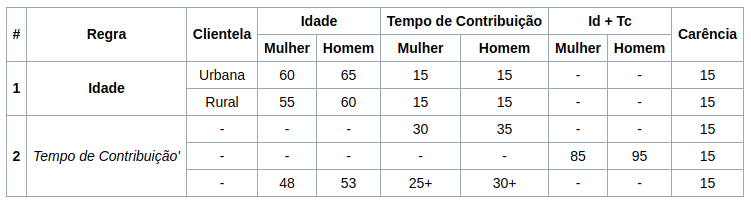
\includegraphics [scale=0.42]{./Figures/comoe}
     % \caption {Estimativa de dispositivos conectados à Internet.}
  		%\label{fig:arq-imuno}
  	\end{center}
  \end{figure}
  \textbf{Fator Previdenciário}
  	\begin{center}
    $f = \frac{Tc \times a}{Es} \times \left ( 1 + \frac{(Id + Tc \times
    0,31)}{100} \right )$
  	\end{center}
  \begin{itemize}
    \scriptsize
    \item $f$: Fator previdenciário
    \item $Tc$: Tempo de contribuição até o momento da aposentadoria
    \item $Id$: Idade no momento da aposentadoria
    \item $Es$: Expectativa de sobrevida no momento da aposentadoria
  \end{itemize}
\end{frame}

\begin{frame}{Como fica}
  Modalidade Única
  \begin{figure}[h]
  	\begin{center}
      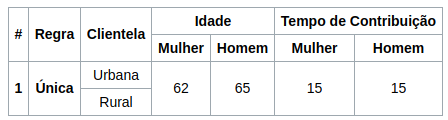
\includegraphics [scale=0.6]{./Figures/comofica}
     % \caption {Estimativa de dispositivos conectados à Internet.}
  		%\label{fig:arq-imuno}
  	\end{center}
  \end{figure}
\end{frame}

%\begin{frame}
%  \begin{block}{}
%    \begin{itemize}
%      \item
%    \end{itemize}
%  \end{block}
%\end{frame}

%\begin{frame}
%  \begin{block}{}
%  \end{block}
%\end{frame}

%\begin{frame}
%  \begin{figure}[h]
%  	\begin{center}
%      \includegraphics [scale=0.3]{./Figures/Device-Estimates}
%     % \caption {Estimativa de dispositivos conectados à Internet.}
%  		%\label{fig:arq-imuno}
%  	\end{center}
%  \end{figure}
%\end{frame}

%\begin{frame}{Redes de Acesso}
%	\begin{figure}[!htb]
%		\centering
%		\subfloat[DSL]{
%			\includegraphics[height=3.5cm]{./Figures/DSLaccess}
%			\label{figdroopy}}
%		\quad %espaco separador
%		\subfloat[Cable]{
%			\includegraphics[height=3.5cm]{./Figures/CableAccess}
%			\label{figsnoop}}
%		%\caption{Subfiguras}
%		%\label{fig01}
%	\end{figure}
%\end{frame}

%\begin{frame}[fragile]
%\scriptsize
%\begin{verbatim}
%\end{verbatim}
%\end{frame}

%\begin{frame}{\textit{Socket Programming with TCP}}
%\scriptsize
%\lstinputlisting[language=Python, caption={TCP Server.}]{./code/upperServer/TCPserver.py}
%\end{frame}



\section[Proposta]{Trabalho Proposto}
\frame{\tableofcontents[currentsection]}
\begin{frame}
  \begin{block}{}
    \begin{itemize}
      \item Em 2017, Carlos Patrick \cite{patrick} demonstrou que os dados
      oficiais do governo referentes à previdência social apresentam
      \textbf{projeções} \alert{viesadas no curto prazo}, e com \alert{erros
elevados no longo prazo}.
      \item Alertou ainda para a \alert{impossibilidade de reprodução dos
resultados} das Leis de Diretrizes orçamentárias (LDOs) de 2012 e 2018
      \begin{itemize}
        \item Falta de tansparência nos dados oficiais
        \item Falta de tansparência na metodologia
      \end{itemize}
    \end{itemize}
  \end{block}
\end{frame}

\begin{frame}
  \begin{block}{CPI da Previdência}
    \begin{itemize}
      \item Após a publicação da tese do Prof. Carlos Patrick, foram
      disponibilizados pelo governo os microdados (dados não agregados) da base
      utilizada naquela pesquisa
      \item Torna-se possível avaliar as variáveis que sofrerão mudanças com a
      reforma:
      \begin{itemize}
        \item  Melhores análise
        \item  Melhores projeções
        \item  Exercício de novos modelos
      \end{itemize}
    \end{itemize}
  \end{block}
\end{frame}

\begin{frame}
  \begin{block}{Objetivos}
    \begin{itemize}
      \item Reproduzir o modelo de projeção oficial utilizando os microdados
      \begin{itemize}
        \item Ratificar o grau de incerteza obtido nos dados agregados
        \item \alert{Novas propostas de reforma}
      \end{itemize}
      \item Simular a reforma da previdência com os dados históricos
      \item Propor um novo modelo de projeção de longo prazo para a previdência
      social no Brasil
    \end{itemize}
  \end{block}
\end{frame}

%\begin{frame}
%  \begin{block}{}
%    \begin{itemize}
%      \item
%    \end{itemize}
%  \end{block}
%\end{frame}

%\begin{frame}
%  \begin{block}{}
%  \end{block}
%\end{frame}

%\begin{frame}
%  \begin{figure}[h]
%  	\begin{center}
%      \includegraphics [scale=0.3]{./Figures/Device-Estimates}
%     % \caption {Estimativa de dispositivos conectados à Internet.}
%  		%\label{fig:arq-imuno}
%  	\end{center}
%  \end{figure}
%\end{frame}

%\begin{frame}{Redes de Acesso}
%	\begin{figure}[!htb]
%		\centering
%		\subfloat[DSL]{
%			\includegraphics[height=3.5cm]{./Figures/DSLaccess}
%			\label{figdroopy}}
%		\quad %espaco separador
%		\subfloat[Cable]{
%			\includegraphics[height=3.5cm]{./Figures/CableAccess}
%			\label{figsnoop}}
%		%\caption{Subfiguras}
%		%\label{fig01}
%	\end{figure}
%\end{frame}

%\begin{frame}[fragile]
%\scriptsize
%\begin{verbatim}
%\end{verbatim}
%\end{frame}

%\begin{frame}{\textit{Socket Programming with TCP}}
%\scriptsize
%\lstinputlisting[language=Python, caption={TCP Server.}]{./code/upperServer/TCPserver.py}
%\end{frame}




\section[Resultados]{Simulações e Resultados}

\subsection{Modelagem}
\frame{\tableofcontents[currentsection]}
\begin{frame}
  Modelagem
\end{frame}

\begin{frame}{Bases de dados}
  \begin{block}{Base de dados da previdência}
    \begin{itemize}
      \item Disponibilizado no site \alert{\underline{\url{https://legis.senado.leg.br}}}
      \item Dados relacionados a benefícios (\alert{aposentadorias} e \alert{pensões}) concedidos pelo RGPS no período de 1995-2016
      \item Dois documentos disponibilizados
      \begin{itemize}
        \item Doc090/Mídia018 e Doc097/Mídia019
      \end{itemize}
    \end{itemize}
  \end{block}
    
  \begin{block}{Pré-processamento dos dados}
    \begin{itemize}
      \item Utilização da ferramenta \alert{Pentaho Data Integration} para a organização do banco de dados
      \item Modelo de \alert{Data Warehouse} empregado na modelagem
      \item Utilização de um servidor local PostgreSQL 
    \end{itemize}
  \end{block}
\end{frame}

\begin{frame}{Origem dos Dados}
  \begin{figure}[h]
  	\begin{center}
      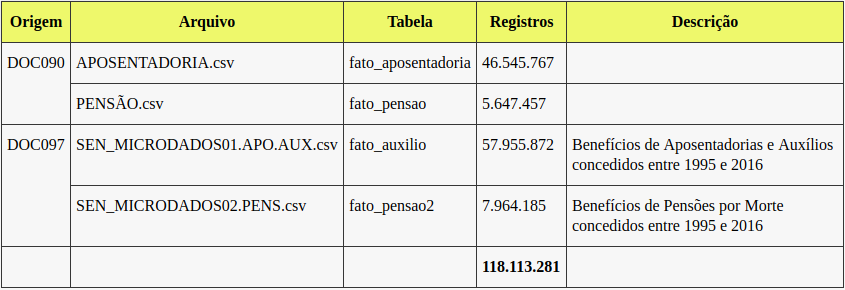
\includegraphics [scale=0.48]{./Figures/table1}
     % \caption {Estimativa de dispositivos conectados à Internet.}
  		%\label{fig:arq-imuno}
  	\end{center}
  \end{figure}
  
  \begin{block}{}
    \begin{itemize}
      \item Análise da tabela \alert{fato\_auxilio/DOC097}
      \item Contém as informações relevantes e necessárias para a proposta em questão
    \end{itemize}
  \end{block}
\end{frame}

\begin{frame}
  \begin{block}{}
    \begin{itemize}
      \item \alert{14 variáveis} relacionadas aos beneficiarios
      \begin{itemize}
        \item Informações pessoais e relacionadas aos benefícios
        % \item Informações relacionadas aos benefícios
      \end{itemize}
    \end{itemize}
  \end{block}    
  
  \begin{table}[]
    \begin{tabular}{|l|l|}
      \hline
      {\tiny CAMPO}           & {\tiny DESCRIÇÃO}                                               \\ \hline
      {\tiny ESPECIE}         & {\tiny Espécie do Benefício}                                    \\ \hline
      {\tiny DIB}             & {\tiny Data de Início do Benefício}                             \\ \hline
      {\tiny DDB}             & {\tiny Data de Despacho do Benefício}                           \\ \hline
      {\tiny MOT\_CESSACAO}   & {\tiny Motivo de Cessação}                                      \\ \hline
      {\tiny ULT\_COMPET\_MR} & {\tiny Competência de Cálculo da Última Mensalidade Reajustada} \\ \hline
      {\tiny VL\_MR}          & {\tiny Valor da Última Mensalidade Reajustada}                  \\ \hline
      {\tiny DT\_NASC}        & {\tiny Data de Nascimento do Titular}                           \\ \hline
      {\tiny VL\_RMI}         & {\tiny Valor da Renda Mensal Inicial}                           \\ \hline
      {\tiny CLIENTELA}       & {\tiny Clientela}                                               \\ \hline
      {\tiny SEXO}            & {\tiny Sexo do Titular}                                         \\ \hline
      {\tiny SITUACAO}        & {\tiny Situação do Benefício }                                  \\ \hline
      {\tiny DT\_OBITO}       & {\tiny Data de Óbito}                                           \\ \hline
      {\tiny TEMP\_CONTRIB}   & {\tiny Tempo de Contribuição (em anos) do Titular}              \\ \hline
      {\tiny IDADE\_DIB}      & {\tiny Idade na DIB do Titular}                                 \\ \hline
    \end{tabular}
  \end{table}
\end{frame}

\begin{frame}
  \begin{block}{Pré-processamento dos dados}
    \begin{itemize}
      \item Utilização da ferramenta \alert{Pentaho Data Integration} para a organização do banco de dados
      \item Modelo de \alert{Data Warehouse} empregado na modelagem
      \item Utilização de um servidor local PostgreSQL 
    \end{itemize}
  \end{block}
  
  \begin{figure}[h]
  	\begin{center}
      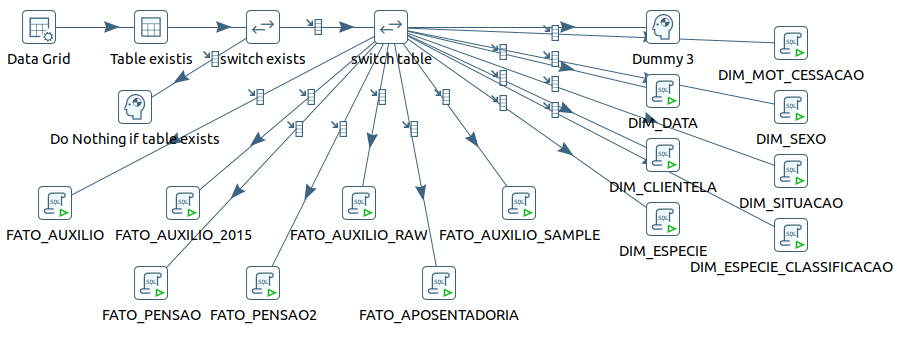
\includegraphics [scale=0.34]{./Figures/etl}
     % \caption {Estimativa de dispositivos conectados à Internet.}
  		%\label{fig:arq-imuno}
  	\end{center}
  \end{figure}
\end{frame}

\begin{frame}{Bases de dados}
  \begin{block}{INSS - Anuário Estatístico da Previdência Social}
    \begin{itemize}
      \item Dados Agregados
      \begin{itemize}
        \item Benefícios
        \item População 2013/2014/2015
      \end{itemize}
    \end{itemize}
  \end{block}
  \begin{figure}[h]
  	\begin{center}
      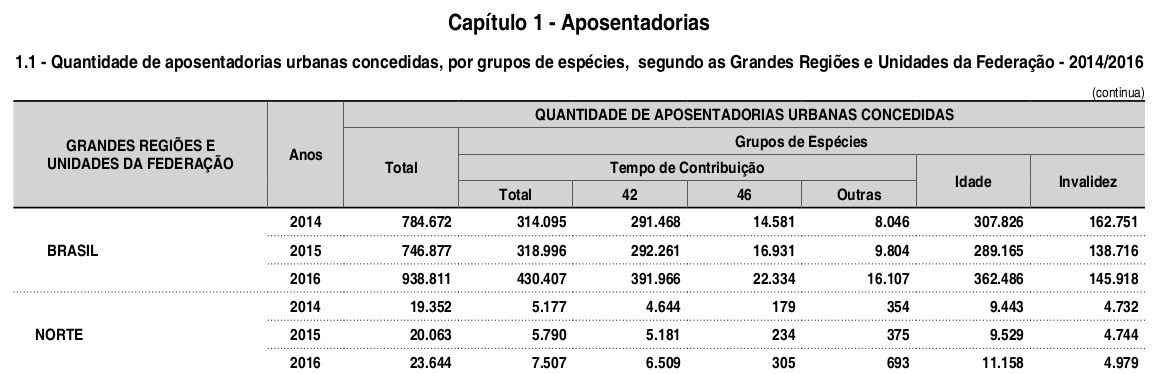
\includegraphics [scale=0.27]{./Figures/aeps01}
     % \caption {Estimativa de dispositivos conectados à Internet.}
  		%\label{fig:arq-imuno}
  	\end{center}
  \end{figure}
\end{frame}

\begin{frame}{Bases de dados}
  \begin{block}{Projeção da População Brasileira}
    \begin{itemize}
      \item Taxas anuais de crescimento da população até 2060
    \end{itemize}
  \end{block}
  \begin{figure}[h]
  	\begin{center}
      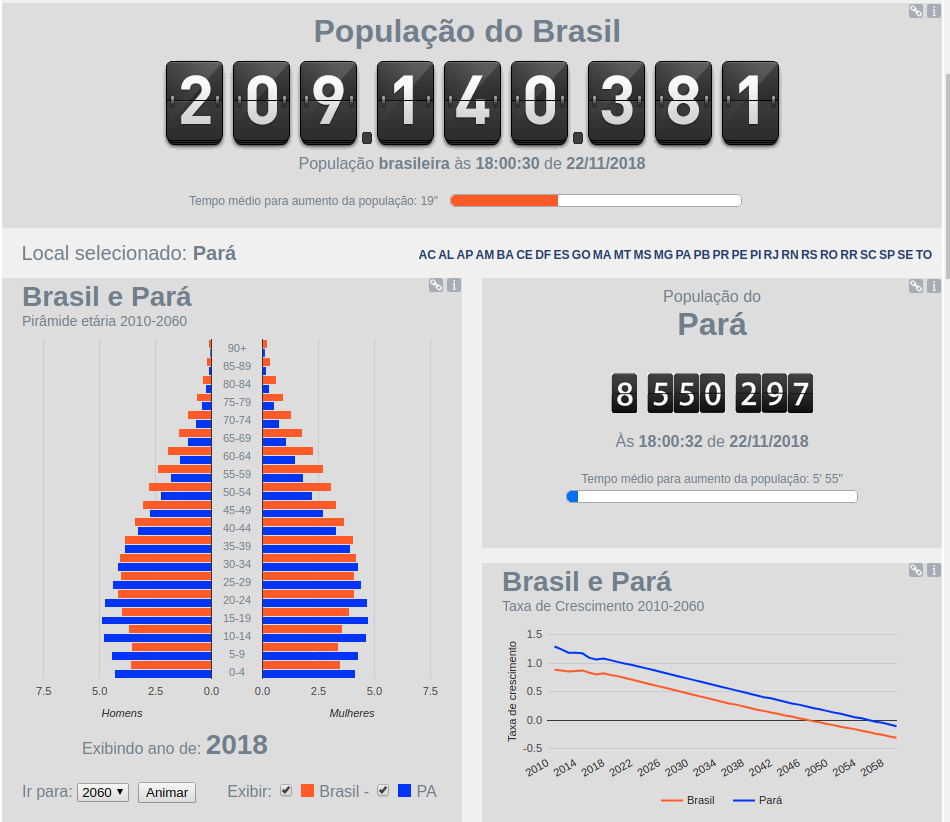
\includegraphics [scale=0.23]{./Figures/ibge-pop}
     % \caption {Estimativa de dispositivos conectados à Internet.}
  		%\label{fig:arq-imuno}
  	\end{center}
  \end{figure}
\end{frame}

\begin{frame}{Modelos de Projeção de Longo Prazo}
  \begin{block}{}
    \begin{itemize}
      \item Avaliação lida com eventos incertos e complexos sistemas
      interligados
      \item Modelo: representação simplificada da realidade, devendo
      considerar aspectos:
      \begin{itemize}
        \item demográficos
        \item financeiros
        \item institucionais
        \item jurídicos
      \end{itemize}
      \item Cálculo exige utilização de dados estatísticos confiáveis
    \end{itemize}
  \end{block}
\end{frame}

\begin{frame}{Variáveis em Modelos de Projeção}
\scriptsize
  \begin{block}{Variáveis Demográficas}
    \begin{itemize}
      \item Taxa de fecundidade
      \item Taxa de natalidade
      \item Expectativa de vida
      \item Taxa de migração
      \item Taxa de urbanização
    \end{itemize}
  \end{block}
  \pause
  \begin{block}{Variáveis Econômicas}
    \begin{itemize}
      \item Reajuste dos salários
      \item Inflação
      \item Taxas de juros
      \item Desemprego
      \item Produtividade
      \item Formalização
      \item Crescimento Econômico
    \end{itemize}
  \end{block}
\end{frame}

\begin{frame}{Variáveis em Modelos de Projeção}
  \begin{block}{Variáveis Previdenciárias}
    \begin{itemize}
      \item Alíquotas de contribuição
      \item Probabilidades de entrada no sistema
      \item Probabilidades de saída do sistema
      \item Reajuste dos benefícios
      \item Valores médios dos benefícios
    \end{itemize}
  \end{block}
\end{frame}

\begin{frame}{Modelos de Projeção}
  \begin{block}{1o Modelo Oficial do Governo Brasileiro}
    \begin{itemize}
      \item Criado no final da década de 90
      \item Permite projeção de receitas e despesas até a data de projeção da
      população (IBGE)
      \item Utilizado na elaboração de metas fiscais (LDO)
    \end{itemize}
  \end{block}

  \begin{block}{2o Modelo Oficial}
    \begin{itemize}
      \item Criado em 2016
      \item Visa melhor aderência a legislação vigente
      \item Modela de forma mais precisa os benefícios
      \item Mais complexo
    \end{itemize}
  \end{block}
\end{frame}

\begin{frame}{1o Modelo}
  \begin{block}{Considerações}
    \begin{itemize}
      \item Modelo determinístico
      \item  A LDO de 2017, não descreve quais benefícios são usados no modelo
      \item  A simplicidade do modelo o torna fácil de implementar, mas abstrair
      todos os benefícios em poucas equações afeta consideravelmente a
      precisão dos resultados
    \end{itemize}
  \end{block}
\end{frame}

\begin{frame}{1o Modelo - Estoque}
  \begin{block}{Estoque de Benefícios}
    \begin{itemize}
      \item Para cálculo das despesas, precisa-se calcular os \alert{benefícios
      ativos} no referido ano
      \item Calculado pelo método de fluxos, onde a concessão e cessação de
      benefícios são estimadas e utilizadas para definição do estoque
    \end{itemize}
  \end{block}
\end{frame}

\begin{frame}{1o Modelo - Estoque}
  \begin{block}{Fluxos de Concessão}
    \begin{center}
      $Fe(i,t,s,c,k) = P(i,t,s,c) \times Pe(i,t,s,c,k)$
    \end{center}
  \end{block}
  \begin{block}{Probabilidade de Entrada}
    \begin{center}
      $Pe(i,t,s,c,k) = \frac{concessoes(i,t,s,c,k)}{P(i,t,s,c)}$
    \end{center}
  \end{block}
  \begin{block}{Probabilidade de Sobrevivência}
    \begin{center}
      $Ps (i, t, s) = \frac{P(i+1, t+1, s)}{P(i,t,s)}$
    \end{center}
  \end{block}
\end{frame}

\begin{frame}{1o Modelo - Estoque}
  \begin{block}{Estoque de Benefício}
    \begin{center}
      $Eb(i, t, s, c, k) = Eb(i-1, t-1, s, c, k) \times Ps(i,s,c,k) \times
      Fe(i, t ,s, c, k)$
    \end{center}
  \end{block}
  \begin{block}{Estoque Total de Benefícios}
    \begin{center}
      $\sum_i \sum_s \sum_c \sum_k Eb(i,t,s,c,k)$
    \end{center}
  \end{block}
\end{frame}

\begin{frame}{1o Modelo - Despesa}
  \begin{block}{Despesa com Benefícios}
    Calculada a partir do estoque e do valor médio dos benefícios:
      \begin{center}
  \scriptsize
$Db(i,t,s,c,k) =$
$[Eb(i-1, t-1, s, c, k) \times Ps(i,s,c,k) \times Vmb(i,t,s,c,k)] + [Fe(i, t ,s, c, k) \times Vmbe(i,t,s,c,k)]$
      \end{center}
  \end{block}
  \scriptsize
    Onde:
    \begin{itemize}
      \item $Vmb$ é o valor médio atual do benefício (já concedido) pago
      \item $Vmbe$ é o valor médio do benefício (projetado) pago
    \end{itemize}
\end{frame}

\begin{frame}{1o Modelo - Receita}
  \begin{block}{Número de contribuintes}
  \scriptsize
      \begin{center}
      $\sum_i \sum_s \sum_c C(i,t,s,c) =$ \\
       $\sum_i \sum_s \sum_c P(i,t,s,c) \times Part(i,t,s,c) \times [1-Desemp(i,t,s,c)] \times d(i,t,s,c)$
      \end{center}
    %\end{itemize}
  \end{block}
  \scriptsize
    Onde:
    \begin{itemize}
      \item $C$ é o estoque de contibuintes
      \item $P$ é a população
      \item $Part$ é a taxa de participação na força de trabalho
      \item $Desemp$ é a taxa de desemprego
      \item $d$ é a densidade da contribuição (proporção de meses de contribuição do empregado no ano, onde $d=1$ significa 12 meses de contribuição
    \end{itemize}
\end{frame}

\begin{frame}{1o Modelo - Receita}
  \begin{block}{Valor da Receita $R$ no ano $t$}
  \scriptsize
      \begin{center}
    $R_t = \sum_i \sum_s \sum_c C(i,t,s,c) \times [al_{trab} \times \text{Min}(Teto, S_a(i,t,s,c)) + al_{emp} \times S_a(i,t,s,c)]$
      \end{center}
    %\end{itemize}
  \end{block}
  \scriptsize
    Onde:
    \begin{itemize}
      \item $al_{trab}$ é a alíquota de contribuição paga pelo trabalhador
      \item $al_{emp}$ é a alíquota de contribuição paga pelo empregador
      \item $Teto$ é o limite de contribuição (maior valor sobre o qual a alíquota pode incidir)
      \item $S_a$ é o saláro do empregado
    \end{itemize}
\end{frame}

%\begin{frame}
%  \begin{block}{}
%    \begin{itemize}
%      \item
%    \end{itemize}
%  \end{block}
%\end{frame}

%\begin{frame}
%  \begin{block}{}
%  \end{block}
%\end{frame}

%\begin{frame}
%  \begin{figure}[h]
%  	\begin{center}
%      \includegraphics [scale=0.3]{./Figures/Device-Estimates}
%     % \caption {Estimativa de dispositivos conectados à Internet.}
%  		%\label{fig:arq-imuno}
%  	\end{center}
%  \end{figure}
%\end{frame}

%\begin{frame}{Redes de Acesso}
%	\begin{figure}[!htb]
%		\centering
%		\subfloat[DSL]{
%			\includegraphics[height=3.5cm]{./Figures/DSLaccess}
%			\label{figdroopy}}
%		\quad %espaco separador
%		\subfloat[Cable]{
%			\includegraphics[height=3.5cm]{./Figures/CableAccess}
%			\label{figsnoop}}
%		%\caption{Subfiguras}
%		%\label{fig01}
%	\end{figure}
%\end{frame}

%\begin{frame}[fragile]
%\scriptsize
%\begin{verbatim}
%\end{verbatim}
%\end{frame}

%\begin{frame}{\textit{Socket Programming with TCP}}
%\scriptsize
%\lstinputlisting[language=Python, caption={TCP Server.}]{./code/upperServer/TCPserver.py}
%\end{frame}


\subsection{Simulações}
\frame{\tableofcontents[currentsection]}
\begin{frame}
  Simulações
\end{frame}

\begin{frame}
  Reforma da previdência
\end{frame}

\begin{frame}
  Estoque de benefícios
\end{frame}

%\begin{frame}
%  \begin{block}{}
%    \begin{itemize}
%      \item
%    \end{itemize}
%  \end{block}
%\end{frame}

%\begin{frame}
%  \begin{block}{}
%  \end{block}
%\end{frame}

%\begin{frame}
%  \begin{figure}[h]
%  	\begin{center}
%      \includegraphics [scale=0.3]{./Figures/Device-Estimates}
%     % \caption {Estimativa de dispositivos conectados à Internet.}
%  		%\label{fig:arq-imuno}
%  	\end{center}
%  \end{figure}
%\end{frame}

%\begin{frame}{Redes de Acesso}
%	\begin{figure}[!htb]
%		\centering
%		\subfloat[DSL]{
%			\includegraphics[height=3.5cm]{./Figures/DSLaccess}
%			\label{figdroopy}}
%		\quad %espaco separador
%		\subfloat[Cable]{
%			\includegraphics[height=3.5cm]{./Figures/CableAccess}
%			\label{figsnoop}}
%		%\caption{Subfiguras}
%		%\label{fig01}
%	\end{figure}
%\end{frame}

%\begin{frame}[fragile]
%\scriptsize
%\begin{verbatim}
%\end{verbatim}
%\end{frame}

%\begin{frame}{\textit{Socket Programming with TCP}}
%\scriptsize
%\lstinputlisting[language=Python, caption={TCP Server.}]{./code/upperServer/TCPserver.py}
%\end{frame}


\section{Conclusões}
\frame{\tableofcontents[currentsection]}
\begin{frame}
  \begin{block}{}
    \begin{itemize}
      \item
    \end{itemize}
  \end{block}
\end{frame}

%\begin{frame}
%  \begin{block}{}
%    \begin{itemize}
%      \item
%    \end{itemize}
%  \end{block}
%\end{frame}

%\begin{frame}
%  \begin{block}{}
%  \end{block}
%\end{frame}

%\begin{frame}
%  \begin{figure}[h]
%  	\begin{center}
%      \includegraphics [scale=0.3]{./Figures/Device-Estimates}
%     % \caption {Estimativa de dispositivos conectados à Internet.}
%  		%\label{fig:arq-imuno}
%  	\end{center}
%  \end{figure}
%\end{frame}

%\begin{frame}{Redes de Acesso}
%	\begin{figure}[!htb]
%		\centering
%		\subfloat[DSL]{
%			\includegraphics[height=3.5cm]{./Figures/DSLaccess}
%			\label{figdroopy}}
%		\quad %espaco separador
%		\subfloat[Cable]{
%			\includegraphics[height=3.5cm]{./Figures/CableAccess}
%			\label{figsnoop}}
%		%\caption{Subfiguras}
%		%\label{fig01}
%	\end{figure}
%\end{frame}

%\begin{frame}[fragile]
%\scriptsize
%\begin{verbatim}
%\end{verbatim}
%\end{frame}

%\begin{frame}{\textit{Socket Programming with TCP}}
%\scriptsize
%\lstinputlisting[language=Python, caption={TCP Server.}]{./code/upperServer/TCPserver.py}
%\end{frame}



%\section{Referências}
%\frame{\tableofcontents[currentsection]}

\begin{frame}[allowframebreaks]{Referências}
% \bibliography{../referencias}

\begin{thebibliography}{10}
		\bibitem{reformarparaexcluir}[1]
      Gentil, Denise Lobato.
      \newblock Previdência: reformar para excluir?
      \newblock Seminário "Reforma da Previdência: Análise da PEC 287/2016",
      2017.
		\bibitem{patrick}[2]
			Carlos Silva
			\newblock Uma Metodologia para Aferição de Acurácia de Modelos de
      Projeção de Longo Prazo para a Prividência Social no Brasil
			\newblock Tese de Doutorado, UFPa, 2017.
		%\bibitem{class}[2]
		%	Author name
		%	\newblock Title.
		%	\newblock Conference, 2018.
\end{thebibliography}
\end{frame}

\begin{frame}{Dúvidas?}
  \begin{figure}[h]
  	\begin{center}
      
\includegraphics [scale=0.4]{./Figures/duvida}
      %\caption {Modelagem Geral do Sistema Imuno.}
  		%\label{fig:arq-imuno}
  	\end{center}
  \end{figure}
\end{frame}

%\begin{frame}
%	\begin{block}{}
%		\begin{center}
%			\textbf{Obrigado pela aten\c{c}\~{a}o!}
%		\end{center}
%	\end{block}
%	\begin{itemize}
%  		\item andresp@lasca.ic.unicamp.br
%  	\end{itemize}
%	\vspace{2cm}
%\end{frame}


\end{document}
